\documentclass[10pt, letterpaper, conference, final, twocolumn]{ieeeconf}
\IEEEoverridecommandlockouts
\overrideIEEEmargins

%\usepackage{mathpazo}
% packages
\usepackage{amsmath, amsfonts, amssymb, bm, enumerate, url}%, flushend}
\usepackage[boxruled, vlined, linesnumbered]{algorithm2e}
\usepackage[usenames, dvipsnames]{color}
\usepackage[pdftex, xetex]{graphicx}
\usepackage[font={small}]{caption}
\usepackage{float, colortbl, tabularx, multirow, subfig, environ}
\usepackage{pgf, tikz}
\usetikzlibrary{arrows,automata}
\usepackage[normalem]{ulem}

\usepackage[bookmarks=true]{hyperref}
\hypersetup{
colorlinks=true, linkcolor=red, citecolor=blue, filecolor=magenta, urlcolor=blue
%linkcolor=black, citecolor=black, filecolor=black, urlcolor=black
}
\usepackage{url, cite}

% macros
\providecommand{\abs}[1]{\ensuremath \left| #1 \right|}
\providecommand{\norm}[1]{\ensuremath \lVert#1\rVert}
\providecommand{\given}{\, \vert \,}
\providecommand{\cal}[1]{\ensuremath \mathcal{#1}}
\providecommand{\qed}{\hfill \mbox{\raggedright \rule{0.1in}{0.1in} } }

\providecommand{\aeq}[1]{\begin{align} #1 \end{align}}
\providecommand{\aeqs}[1]{\begin{align*} #1 \end{align*}}
\providecommand{\beq}[1]{\begin{equation}#1\end{equation}}
\providecommand{\beqs}[1]{\begin{equation*}#1\end{equation*}}
\providecommand{\trm}[1]{\ensuremath \textrm{#1}}
\providecommand{\enum}[2]{\begin{enumerate}[#1]{#2}\end{enumerate}}
\providecommand{\ilist}[1]{\begin{itemize}{#1}\end{itemize}}
\providecommand{\ag}[1]{\ensuremath \left\langle#1\right\rangle}
\providecommand{\bee}{\begin{enumerate}}
\providecommand{\eee}{\end{enumerate}}
\providecommand{\bm}[1]{\begin{bmatrix}#1\end{bmatrix}}

\usepackage{theorem}
\newtheorem{theorem}{Theorem}
\newtheorem{proposition}[theorem]{Proposition}
\newtheorem{lemma}[theorem]{Lemma}
\newtheorem{corollary}[theorem]{Corollary}
\newtheorem{problem}[theorem]{Problem}
%\theoremstyle{definition}
\newtheorem{definition}[theorem]{Definition}
\newtheorem{example}[theorem]{Example}
\newtheorem{note}[theorem]{Note}
\newtheorem{remark}[theorem]{Remark}
%\theoremstyle{plain}
\newtheorem{assumption}[theorem]{Assumption}

\newcommand{\PP}{\ensuremath \mathbb{P}}
\newcommand{\EE}{\ensuremath \mathbb{E}}

% margins
\setlength{\marginparwidth}{0.6in}
\definecolor{darkgreen}{rgb}{0,0.6,0} \newcommand{\dg}{\color{darkgreen}}
\definecolor{fullred}{rgb}{0.85,.0,.1} \newcommand{\fr}{\color{fullred}}
\definecolor{darkblue}{rgb}{0,0,1.0} \newcommand{\db}{\color{darkblue}}
\definecolor{brown}{rgb}{0.54,.27,0} \newcommand{\br}{\color{brown}}

\newcommand{\pcm}[2]{{\dg #1}\marginpar{\tiny\noindent{\raggedright{\dg[PC]}\br{ #2} \par}}}
\newcommand{\vsm}[2]{{\fr #1}\marginpar{\tiny\noindent{\raggedright{\dg[VS]}\db{ #2} \par}}}
%\renewcommand{\margin}[2]{#1}
\newcommand{\ignore}[1]{}

% save space
\newcommand{\algsize}{\footnotesize}
\setlength{\floatsep}{0.05in}
\setlength{\textfloatsep}{0.1in}
\setlength{\intextsep}{0.05in}
\setlength{\belowcaptionskip}{0.01in}
\setlength{\abovecaptionskip}{0.1in}
\setlength{\abovedisplayskip}{0.08in}
\setlength{\belowdisplayskip}{0.08in}

\begin{document}
\title{\bf Twitter-based Mood Evaluation
	\thanks{$^*$Chemical Engingeering Department, MIT. Email: \href{mailto:vishnusr@mit.edu}{vishnusr@mit.edu}}
	\thanks{$^\dag$Laboratory of Information and Decision Systems, MIT. Email: \href{mailto:pratikac@mit.edu}{pratikac@mit.edu}}
}
\author{Vishnu Sresht$^*$ \qquad Pratik Chaudhari$^\dag$}
\maketitle

\begin{abstract}
By providing a convenient, readily-accessible way to reach out to a global audience, twitter has revolutionized the way we broadcast our feelings to the rest of the world. In addition to its empowerment of the diva within us all, Twitter's meteoric rise in popularity has enabled every one of us to listen to the voices of millions and comprehend mankind's \textit{zeitgest} at an uprecedented resolution. However, the deluge of verbiage unleashed by Twitter's ubiquitous usage must be tamed before its wealth of information can be exploited for sociologically-beneficial research. In this project, we attempt to survey, compare and contrast machine learning techniques for one particular form of large-scale tweet analysis - that of determining `how positive people feel' at any given moment through the sentiment analysis of their tweets. To this end, we also introduce a novel source of already classified text corpora for use as training data. Sites like \href{http://mylifeisg.com}{My Life Is G} and \href{http://fmylife.com}{FML} are a hiherto unutilized source of crowd-curated, well classified training data of text snippets of appropriate length. In this paper, we intend to study the relative efficacies of several commonly employed classification algorithms, including Naive Bayes, Support Vector Machines, and K-Nearest Neighbor classifiers when applied to the task of of detecting the mood of the nation on a real-time basis.
\end{abstract}

\section{Introduction}
\label{sec:intro}

\section{Scraping data}
\label{sec:data}

\begin{figure}[!htp]
\centering
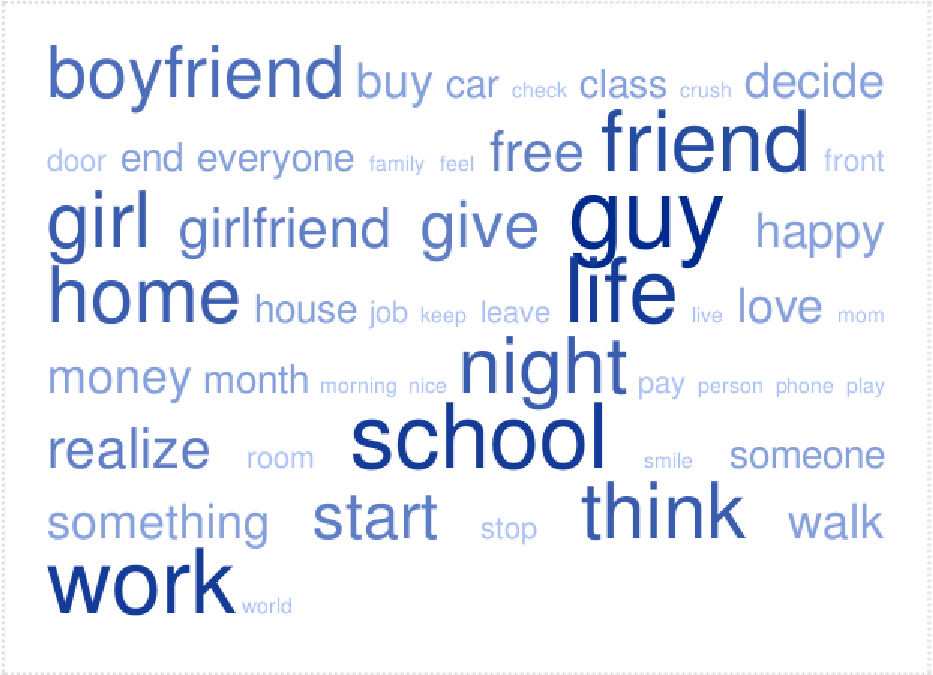
\includegraphics[width= 0.9 \columnwidth]{fig/pos_cloud}
\caption{Word cloud for documents with positive sentiment}
\label{fig:pos_cloud}
\end{figure}
%
\begin{figure}[!htp]
\centering
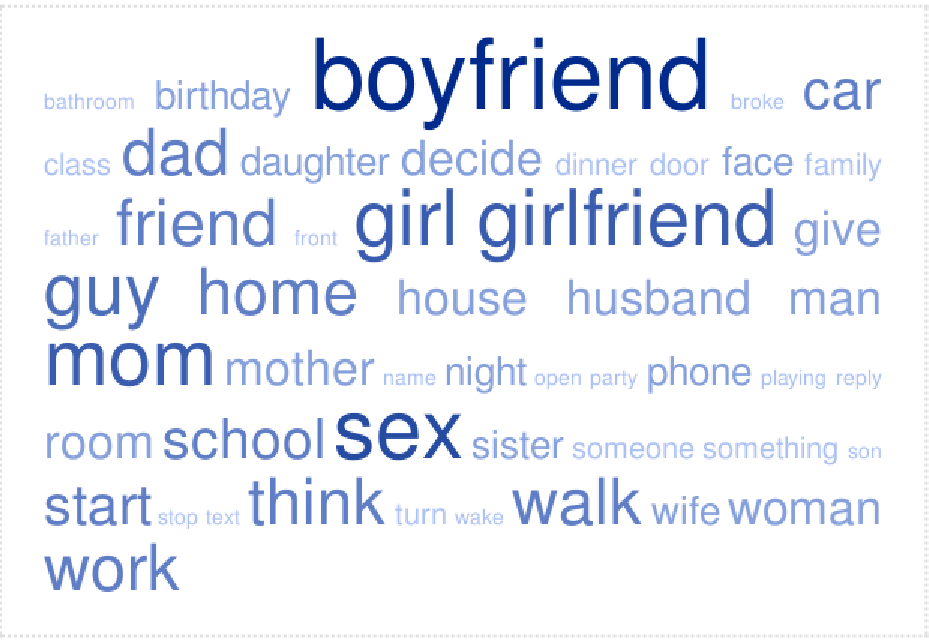
\includegraphics[width= 0.9 \columnwidth]{fig/neg_cloud}
\caption{Word cloud for documents with negative sentiment}
\label{fig:neg_cloud}
\end{figure}

\section{Feature representation}
\label{sec:features}

We employ four different feature representations:
\enum{1.}{
\item Word frequency (WF)
\item Information gain (IG)
\item Gain ratio (GR)
\item Term frequency and inverse document frequency (TF-IDF)
}

\subsection{Word Frequency}
\label{ssec:wf}

\subsection{Information Gain}
\label{ssec:ig}

\subsection{Gain Ratio}
\label{ssec:gr}

\subsection{TF-IDF}
\label{ssec:tfidf}

\section{Preliminary results}
\label{sec:prelim}

This section uses the feature representation created in Sec.~\ref{sec:features} and shows an analysis of various algorithms and features on the data. 
In addition to this, we analyse the data using four different algorithms,
\enum{1.}{
\item Support Vector Machine
\item Principle component analysis (PCA) with SVM
\item Adaboost
\item Naive Bayes classifier
}

\section{Latent topics}
\label{sec:latent}

The previous section demonstrated the performance of various classifers on the feature representations obtained from the data. This section builds upon the idea that words in a document are results of a few latent topics. In other words, rather than training a classifer to distinguish between words, we train it to distinguish between latent topics. The analysis in this section is inspired by~\cite{nikolov2012nonparametric}.

This idea has been pursued in literature in a number of different ways. Let us note a popular line of research that introduces supervised learning for topic models~\cite{blei2010supervised}. The idea here is to classify using 

Suppose that for the two classes, $+$ (documents that express positive sentiment) and $-$ (documents that express a negative sentiment), we have a set of latent topics. Let $p = \{ p_1, \ldots, p_m \}$ be the topics that result in words associated with $+$ and $q = \{ q_1, \ldots, q_n \}$ be the topics that result in words associated with $-$. Each sentiment $+$, $-$ is a noisy observation based upon these latent topics. However, we do not know what these topics are and hence we create a simple model based on them.

Denote the words in a document by $s$. Let the probability of generating an observation $s$ from latent topics $p$ be
$$
\PP(s\ \trm{generated from}\ p) \propto e^{-\gamma d(s, p)}
$$
where $d(s,p)$ is some positive definite function that metric and $\gamma$ is a tunable parameter. Note that we need $d(s,p)$ to be symmetric. In our work, we use the Hamming distance between two feature representations as the function $d(\cdot, \cdot)$. We make use of the set of observations, i.e., words in documents to classify a new document. Let $R_+$ be the set of all reference documents that are maked as $+$, $R_-$ is defined similarly. The probability of a new signal $s$ belonging to $+$ is then,

\aeqs{
\PP(+ \given s) &= \sum_{r \in R_+}\ \PP(s\ \trm{in}\ +, s\ \trm{shares a latent source with } r)\\
&= \sum_{r \in R_+} \sum_{j=1}^n \PP(s \trm{ generated by } p_j, r \trm{ generated by } p_j)\\
&\propto  \sum_{r \in R_+} \sum_{j=1}^n \exp(-\gamma[ d(s, p_j) + d(r, p_j)])\\
&\sim \sum_{r \in R_+} \exp \left( -\gamma \min_j [ d(s, p_j) + d(r, p_j)] \right)\\
&\sim \sum_{r \in R_+} \exp \left(-C\ \gamma d(s,r) \right).
}
The second last approximation is obtained as follows: We see that for a large $\gamma$, the summation $\sum_{j=1}^n$ is dominated by the term with the minimum exponent. On the other hand, the last approximation is obtained by noting that the minimum over all terms of the form $[ d(s, p_j) + d(r, p_j)]$ over all signals in $p$ is of the form $C d(s,r)$ for some $C > 0$ and is achieved at $p^* = (s+r)/2$. It is easy to see that this is a valid approximation when the latent source $p_{j^*}$ is close to the global minimizer $p^*$.

We can approximate $\PP(- \given s)$ similarly. The crux of this approach is that we cannot compare observations, i.e., words in documents to latent signals because we do not know them. Instead, we compare words to reference words in the traning data itself and obtain a simple rule for a discriminative classifier. Let $R(s) = \PP(+ \given s)/\PP(- \given s)$ and $\theta$ be a threshold. We classify the observation according to the function $f(s) = \trm{sign}(R(s) - \theta)$. It is clear that $\theta > 1$, we tuned $\theta$ and set its value to $1.25$ because we would like make fewer mistakes while classifying a tweet as $+$ (cite the walmart pregnancy example here).

\section{Conclusions}
\label{sec:conclusions}

\bibliography{writeup}
\bibliographystyle{unsrt}

\end{document}

